\PassOptionsToPackage{unicode=true}{hyperref} % options for packages loaded elsewhere
\PassOptionsToPackage{hyphens}{url}
%
\documentclass[
]{article}
\usepackage{lmodern}
\usepackage{amssymb,amsmath}
\usepackage{ifxetex,ifluatex}
\ifnum 0\ifxetex 1\fi\ifluatex 1\fi=0 % if pdftex
  \usepackage[T1]{fontenc}
  \usepackage[utf8]{inputenc}
  \usepackage{textcomp} % provides euro and other symbols
\else % if luatex or xelatex
  \usepackage{unicode-math}
  \defaultfontfeatures{Scale=MatchLowercase}
  \defaultfontfeatures[\rmfamily]{Ligatures=TeX,Scale=1}
\fi
% use upquote if available, for straight quotes in verbatim environments
\IfFileExists{upquote.sty}{\usepackage{upquote}}{}
\IfFileExists{microtype.sty}{% use microtype if available
  \usepackage[]{microtype}
  \UseMicrotypeSet[protrusion]{basicmath} % disable protrusion for tt fonts
}{}
\makeatletter
\@ifundefined{KOMAClassName}{% if non-KOMA class
  \IfFileExists{parskip.sty}{%
    \usepackage{parskip}
  }{% else
    \setlength{\parindent}{0pt}
    \setlength{\parskip}{6pt plus 2pt minus 1pt}}
}{% if KOMA class
  \KOMAoptions{parskip=half}}
\makeatother
\usepackage{xcolor}
\IfFileExists{xurl.sty}{\usepackage{xurl}}{} % add URL line breaks if available
\IfFileExists{bookmark.sty}{\usepackage{bookmark}}{\usepackage{hyperref}}
\hypersetup{
  pdftitle={CalgaryVotingTrends},
  pdfauthor={L.Doyle},
  pdfborder={0 0 0},
  breaklinks=true}
\urlstyle{same}  % don't use monospace font for urls
\usepackage[margin=1in]{geometry}
\usepackage{color}
\usepackage{fancyvrb}
\newcommand{\VerbBar}{|}
\newcommand{\VERB}{\Verb[commandchars=\\\{\}]}
\DefineVerbatimEnvironment{Highlighting}{Verbatim}{commandchars=\\\{\}}
% Add ',fontsize=\small' for more characters per line
\usepackage{framed}
\definecolor{shadecolor}{RGB}{248,248,248}
\newenvironment{Shaded}{\begin{snugshade}}{\end{snugshade}}
\newcommand{\AlertTok}[1]{\textcolor[rgb]{0.94,0.16,0.16}{#1}}
\newcommand{\AnnotationTok}[1]{\textcolor[rgb]{0.56,0.35,0.01}{\textbf{\textit{#1}}}}
\newcommand{\AttributeTok}[1]{\textcolor[rgb]{0.77,0.63,0.00}{#1}}
\newcommand{\BaseNTok}[1]{\textcolor[rgb]{0.00,0.00,0.81}{#1}}
\newcommand{\BuiltInTok}[1]{#1}
\newcommand{\CharTok}[1]{\textcolor[rgb]{0.31,0.60,0.02}{#1}}
\newcommand{\CommentTok}[1]{\textcolor[rgb]{0.56,0.35,0.01}{\textit{#1}}}
\newcommand{\CommentVarTok}[1]{\textcolor[rgb]{0.56,0.35,0.01}{\textbf{\textit{#1}}}}
\newcommand{\ConstantTok}[1]{\textcolor[rgb]{0.00,0.00,0.00}{#1}}
\newcommand{\ControlFlowTok}[1]{\textcolor[rgb]{0.13,0.29,0.53}{\textbf{#1}}}
\newcommand{\DataTypeTok}[1]{\textcolor[rgb]{0.13,0.29,0.53}{#1}}
\newcommand{\DecValTok}[1]{\textcolor[rgb]{0.00,0.00,0.81}{#1}}
\newcommand{\DocumentationTok}[1]{\textcolor[rgb]{0.56,0.35,0.01}{\textbf{\textit{#1}}}}
\newcommand{\ErrorTok}[1]{\textcolor[rgb]{0.64,0.00,0.00}{\textbf{#1}}}
\newcommand{\ExtensionTok}[1]{#1}
\newcommand{\FloatTok}[1]{\textcolor[rgb]{0.00,0.00,0.81}{#1}}
\newcommand{\FunctionTok}[1]{\textcolor[rgb]{0.00,0.00,0.00}{#1}}
\newcommand{\ImportTok}[1]{#1}
\newcommand{\InformationTok}[1]{\textcolor[rgb]{0.56,0.35,0.01}{\textbf{\textit{#1}}}}
\newcommand{\KeywordTok}[1]{\textcolor[rgb]{0.13,0.29,0.53}{\textbf{#1}}}
\newcommand{\NormalTok}[1]{#1}
\newcommand{\OperatorTok}[1]{\textcolor[rgb]{0.81,0.36,0.00}{\textbf{#1}}}
\newcommand{\OtherTok}[1]{\textcolor[rgb]{0.56,0.35,0.01}{#1}}
\newcommand{\PreprocessorTok}[1]{\textcolor[rgb]{0.56,0.35,0.01}{\textit{#1}}}
\newcommand{\RegionMarkerTok}[1]{#1}
\newcommand{\SpecialCharTok}[1]{\textcolor[rgb]{0.00,0.00,0.00}{#1}}
\newcommand{\SpecialStringTok}[1]{\textcolor[rgb]{0.31,0.60,0.02}{#1}}
\newcommand{\StringTok}[1]{\textcolor[rgb]{0.31,0.60,0.02}{#1}}
\newcommand{\VariableTok}[1]{\textcolor[rgb]{0.00,0.00,0.00}{#1}}
\newcommand{\VerbatimStringTok}[1]{\textcolor[rgb]{0.31,0.60,0.02}{#1}}
\newcommand{\WarningTok}[1]{\textcolor[rgb]{0.56,0.35,0.01}{\textbf{\textit{#1}}}}
\usepackage{graphicx,grffile}
\makeatletter
\def\maxwidth{\ifdim\Gin@nat@width>\linewidth\linewidth\else\Gin@nat@width\fi}
\def\maxheight{\ifdim\Gin@nat@height>\textheight\textheight\else\Gin@nat@height\fi}
\makeatother
% Scale images if necessary, so that they will not overflow the page
% margins by default, and it is still possible to overwrite the defaults
% using explicit options in \includegraphics[width, height, ...]{}
\setkeys{Gin}{width=\maxwidth,height=\maxheight,keepaspectratio}
\setlength{\emergencystretch}{3em}  % prevent overfull lines
\providecommand{\tightlist}{%
  \setlength{\itemsep}{0pt}\setlength{\parskip}{0pt}}
\setcounter{secnumdepth}{-2}
% Redefines (sub)paragraphs to behave more like sections
\ifx\paragraph\undefined\else
  \let\oldparagraph\paragraph
  \renewcommand{\paragraph}[1]{\oldparagraph{#1}\mbox{}}
\fi
\ifx\subparagraph\undefined\else
  \let\oldsubparagraph\subparagraph
  \renewcommand{\subparagraph}[1]{\oldsubparagraph{#1}\mbox{}}
\fi

% set default figure placement to htbp
\makeatletter
\def\fps@figure{htbp}
\makeatother


\title{CalgaryVotingTrends}
\author{L.Doyle}
\date{08/03/2021}

\begin{document}
\maketitle

\hypertarget{calgary-voting-and-demographics}{%
\subsection{Calgary Voting and
Demographics}\label{calgary-voting-and-demographics}}

This is a work in progress and very much still in it's early stages.

This is an exploratory analysis to explore relationshsips between
demographics of a community and their voting tendencies. I will begin by
looking for patterns in age and gender distribution compared to election
results from the 2017 Civic election. After that I may look to add
additional data like provincial and federal voting habits, housing
income, single family versus multi unit housing, historical civic voting
habits, advance voters trends or voters from seniors residence, etc.
Data was downloaded from the City of Calgary's Open Data website.

\hypertarget{assumptions-and-uncertainties}{%
\subsubsection{Assumptions and
uncertainties}\label{assumptions-and-uncertainties}}

Taking community demographic data and comparing it to election results
from that community will not be a perfect match since multiple
communities will feed into a single polling station and certain
demographics are likely over-represented in voters but it will make a
good first approximation.I would also like to do some statistical
analysis on any perceived trends and relationships to see if they are
significant.

\begin{Shaded}
\begin{Highlighting}[]
\KeywordTok{library}\NormalTok{(tidyverse)}
\CommentTok{# load data}
\NormalTok{Elect <-}\StringTok{ }\KeywordTok{read.csv}\NormalTok{(}\StringTok{"./2017_Official_Election_Results_by_Voting_Station.csv"}\NormalTok{)}
\NormalTok{ComDemo <-}\StringTok{ }\KeywordTok{read.csv}\NormalTok{(}\StringTok{"./Civic_Census_by_Community__Age_and_Gender.csv"}\NormalTok{)}
\end{Highlighting}
\end{Shaded}

\hypertarget{civic-census-by-community-age-gender-from-1996-to-2019}{%
\subsubsection{Civic Census by Community, Age, Gender from 1996 to
2019}\label{civic-census-by-community-age-gender-from-1996-to-2019}}

\href{https://data.calgary.ca/Demographics/Civic-Census-by-Community-Age-and-Gender/vsk6-ghca}{link}

\begin{Shaded}
\begin{Highlighting}[]
\NormalTok{GenderReport <-}\StringTok{ }\NormalTok{ComDemo }\OperatorTok
\StringTok{  }\KeywordTok{group_by}\NormalTok{(YEAR) }\OperatorTok
\StringTok{  }\KeywordTok{summarize}\NormalTok{(}\DataTypeTok{males =} \KeywordTok{sum}\NormalTok{(MALES), }\DataTypeTok{females =} \KeywordTok{sum}\NormalTok{(FEMALES)) }\OperatorTok
\StringTok{  }\KeywordTok{print}\NormalTok{()}
\end{Highlighting}
\end{Shaded}

\begin{verbatim}
## # A tibble: 10 x 3
##     YEAR  males females
##  * <int>  <int>   <int>
##  1  1996 767059       0
##  2  1999 422699  419689
##  3  2001 439514  437005
##  4  2004 467530  465965
##  5  2006 497449  494310
##  6  2009 537403  528052
##  7  2011 547782  543154
##  8  2014 594904  600290
##  9  2016 621021  614150
## 10  2019 641938  638369
\end{verbatim}

The above table indicates that there was no gender reporting in the 1996
Civic Census, filter out 1996.

\begin{Shaded}
\begin{Highlighting}[]
\NormalTok{ComDemo <-}\StringTok{ }\NormalTok{ComDemo }\OperatorTok\StringTok{ }\KeywordTok{filter}\NormalTok{(YEAR }\OperatorTok{!=}\StringTok{ "1996"}\NormalTok{)}
\end{Highlighting}
\end{Shaded}

\hypertarget{calgary-civic-election-results.}{%
\subsubsection{2017 Calgary Civic Election
Results.}\label{calgary-civic-election-results.}}

\href{https://data.calgary.ca/Government/2017-Official-Election-Results-by-Voting-Station/atsy-3a4w}{link}.

\hypertarget{election-data-cleaning}{%
\paragraph{Election Data Cleaning}\label{election-data-cleaning}}

Election results include school board trustees we only care about city
councillors and Mayor for now also remove unwanted columns.

\begin{Shaded}
\begin{Highlighting}[]
\NormalTok{Elect <-}\StringTok{ }\NormalTok{Elect }\OperatorTok\StringTok{ }
\StringTok{  }\KeywordTok{filter}\NormalTok{(Office }\OperatorTok\StringTok{ }\KeywordTok{c}\NormalTok{(}\StringTok{"COUNCILLOR"}\NormalTok{, }\StringTok{"MAYOR"}\NormalTok{)) }\OperatorTok
\StringTok{  }\KeywordTok{select}\NormalTok{(}\OperatorTok{-}\NormalTok{Voting.Station.ID)}
\end{Highlighting}
\end{Shaded}

\hypertarget{voting-station-communities}{%
\paragraph{Voting Station
Communities}\label{voting-station-communities}}

Election results are reported by voting station but do not have
communities associated with the voting stations. Demographic data is
reported by community. To join these two datasets I need to get the
communities that the voting stations are in. I did this by loading
``voting station location'' csv
\href{https://data.calgary.ca/Government/Voting-Stations-Effective-October-16-2017-/ps5q-maip}{link}
and ``community boundaries'' shapefile
\href{https://data.calgary.ca/Base-Maps/Community-Boundaries/surr-xmvs}{link}
(downloaded from the city of Calgary) into QGIS and creating an
intersection layer which includes a community column in the voting
stations table. I then exported that layer and imported it into R.

\begin{Shaded}
\begin{Highlighting}[]
\NormalTok{stationsWcomm <-}\StringTok{ }\KeywordTok{read.csv}\NormalTok{(}\StringTok{"./VotingStationsWCommunity.csv"}\NormalTok{)}

\CommentTok{# Get rid of unwanted columns}
\NormalTok{stationsWcomm <-}\StringTok{ }\NormalTok{stationsWcomm }\OperatorTok
\StringTok{  }\KeywordTok{select}\NormalTok{(VSTN_ID, NAME, comm_code, name_}\DecValTok{2}\NormalTok{)}

\CommentTok{# Join stationsWcomm df w the Elect df, match by name rather than stationID as some stations have multiple ID}
\NormalTok{ElectComm <-}\StringTok{ }\NormalTok{Elect }\OperatorTok\StringTok{ }\KeywordTok{left_join}\NormalTok{(stationsWcomm, }\DataTypeTok{by =} \KeywordTok{c}\NormalTok{(}\StringTok{"Voting.Station.Name"}\NormalTok{ =}\StringTok{ "NAME"}\NormalTok{))}

\CommentTok{# investigate the voting stations that don't correspond to a community & how many votes are associated w them}
\NormalTok{NoCommunity <-}\StringTok{ }\KeywordTok{subset}\NormalTok{(ElectComm, }\KeywordTok{is.na}\NormalTok{(comm_code))}
\KeywordTok{sum}\NormalTok{(NoCommunity}\OperatorTok{$}\NormalTok{Votes) }\CommentTok{# votes not associated w a community}
\end{Highlighting}
\end{Shaded}

\begin{verbatim}
## [1] 22694
\end{verbatim}

\begin{Shaded}
\begin{Highlighting}[]
\KeywordTok{sum}\NormalTok{(Elect}\OperatorTok{$}\NormalTok{Votes) }\CommentTok{# total votes;}
\end{Highlighting}
\end{Shaded}

\begin{verbatim}
## [1] 752708
\end{verbatim}

22694/752708 = 3.0\%. 3\% of votes will not be accounted for if I remove
these rows.

\hypertarget{how-are-the-unaccounted-for-votes-classified}{%
\paragraph{How are the unaccounted for votes
classified}\label{how-are-the-unaccounted-for-votes-classified}}

Determine what type of voting stations the votes with no associated
community are from.

\begin{Shaded}
\begin{Highlighting}[]
\KeywordTok{table}\NormalTok{(NoCommunity}\OperatorTok{$}\NormalTok{Voting.Station.Type)  }
\end{Highlighting}
\end{Shaded}

\begin{verbatim}
## 
##    Advance   Hospital    Mail-in    Regular    Special Travelling 
##        172        344         86         16       1025         86
\end{verbatim}

\hypertarget{votes-not-assigned-to-a-voting-station}{%
\subsection{Votes not assigned to a voting
station}\label{votes-not-assigned-to-a-voting-station}}

Try to make some prediction about the demographic of the unassigned
votes and investigate to make sure there is nothing unusual about the
votes before filtering them from the dataset

\begin{Shaded}
\begin{Highlighting}[]
\NormalTok{NoCommunityType <-}\StringTok{ }\NormalTok{NoCommunity }\OperatorTok
\StringTok{  }\KeywordTok{group_by}\NormalTok{(Voting.Station.Type) }\OperatorTok
\StringTok{  }\KeywordTok{summarize}\NormalTok{(}\DataTypeTok{Votes2 =} \KeywordTok{sum}\NormalTok{(Votes))}
            
\NormalTok{NoCommunityType <-}\StringTok{ }\KeywordTok{mutate}\NormalTok{(NoCommunityType, }\DataTypeTok{percent =} \KeywordTok{round}\NormalTok{(Votes2}\OperatorTok{/}\KeywordTok{sum}\NormalTok{(NoCommunityType}\OperatorTok{$}\NormalTok{Votes2)}\OperatorTok{*}\DecValTok{100}\NormalTok{, }\DecValTok{0}\NormalTok{))}
\NormalTok{NoCommunityType}
\end{Highlighting}
\end{Shaded}

\begin{verbatim}
## # A tibble: 6 x 3
##   Voting.Station.Type Votes2 percent
## * <chr>                <int>   <dbl>
## 1 Advance               7030      31
## 2 Hospital              1087       5
## 3 Mail-in               4756      21
## 4 Regular               4157      18
## 5 Special               5193      23
## 6 Travelling             471       2
\end{verbatim}

This table indicates that 23\% of the NoCommunity votes are from a
``special'' Voting.Station.Type which appears to be the designation
given for seniors residence. These votes could be reasonably assigned to
+65 demographic. \textbf{I need to do something with the below table to
compare it to overall voting habits and make sure it all checks out.
Maybe create visuals for each ward comparing unclassified votes to
in-person votes to look for descrepencies}

\begin{Shaded}
\begin{Highlighting}[]
\CommentTok{# Investigate there is nothing unusual about these votes}
\NormalTok{UnaccountedVotes <-}\StringTok{ }\NormalTok{NoCommunity }\OperatorTok
\StringTok{  }\KeywordTok{group_by}\NormalTok{(Office, Ward, Ballot.Name) }\OperatorTok
\StringTok{  }\KeywordTok{summarize}\NormalTok{(}\DataTypeTok{Votes2 =} \KeywordTok{sum}\NormalTok{(Votes)) }\OperatorTok
\StringTok{  }\KeywordTok{arrange}\NormalTok{(}\KeywordTok{desc}\NormalTok{(Votes2), }\DataTypeTok{.by_group =} \OtherTok{TRUE}\NormalTok{) }\OperatorTok
\StringTok{  }\KeywordTok{print}\NormalTok{()}
\end{Highlighting}
\end{Shaded}

\begin{verbatim}
## `summarise()` has grouped output by 'Office', 'Ward'. You can override using the `.groups` argument.
\end{verbatim}

\begin{verbatim}
## # A tibble: 226 x 4
## # Groups:   Office, Ward [29]
##    Office      Ward Ballot.Name           Votes2
##    <chr>      <int> <chr>                  <int>
##  1 COUNCILLOR     1 SUTHERLAND, Ward         653
##  2 COUNCILLOR     1 BLISS TAYLOR, Coral      260
##  3 COUNCILLOR     1 BLATCH, Chris            117
##  4 COUNCILLOR     1 CHRISTENSEN, Cole         53
##  5 COUNCILLOR     1 KHAN, Cam                 35
##  6 COUNCILLOR     2 MAGLIOCCA, Joe           301
##  7 COUNCILLOR     2 WYNESS, Jennifer         242
##  8 COUNCILLOR     2 MAITLAND, Christopher     71
##  9 COUNCILLOR     2 GEORGEOU, George          19
## 10 COUNCILLOR     3 GONDEK, Jyoti            117
## # ... with 216 more rows
\end{verbatim}

\begin{Shaded}
\begin{Highlighting}[]
\CommentTok{## filter out the votes that are not assigned to a community}
\NormalTok{CommunityVotes <-}\StringTok{ }\KeywordTok{subset}\NormalTok{(ElectComm, }\OperatorTok{!}\KeywordTok{is.na}\NormalTok{(comm_code))}
\end{Highlighting}
\end{Shaded}

\hypertarget{ward-11}{%
\subsection{Ward 11}\label{ward-11}}

I started by looking at distribution of votes for Ward 11 City
Councillor. Analysis indicates that 20\% of Ward11 votes were cast in
advance and are thus not associated with a voting station. I will only
be looking at votes associated with a voting station so that I can
compare them with community demographics in phase two. \textbf{I should
come back and look at the vote distribution in advance voters to see if
it matches in-person voting trends if possible.}

\begin{Shaded}
\begin{Highlighting}[]
\CommentTok{# create a df of just Ward11 }
\NormalTok{Ward11 <-}\StringTok{ }\KeywordTok{filter}\NormalTok{(CommunityVotes, Ward }\OperatorTok{==}\StringTok{ "11"}\NormalTok{, Office }\OperatorTok{==}\StringTok{ "COUNCILLOR"}\NormalTok{) }

\CommentTok{# Determine percentage of votes cast in advance in Ward11}
\NormalTok{Ward11Advance <-}\StringTok{ }\NormalTok{Ward11 }\OperatorTok
\StringTok{  }\KeywordTok{group_by}\NormalTok{(Voting.Station.Type) }\OperatorTok
\StringTok{  }\KeywordTok{summarize}\NormalTok{(}\DataTypeTok{Votes2 =} \KeywordTok{sum}\NormalTok{(Votes))}
\NormalTok{Ward11Advance <-}\StringTok{ }\KeywordTok{mutate}\NormalTok{(Ward11Advance, }\DataTypeTok{percent =} \KeywordTok{round}\NormalTok{(Votes2}\OperatorTok{/}\KeywordTok{sum}\NormalTok{(Votes2)}\OperatorTok{*}\DecValTok{100}\NormalTok{,}\DecValTok{0}\NormalTok{))}
\NormalTok{Ward11Advance}
\end{Highlighting}
\end{Shaded}

\begin{verbatim}
## # A tibble: 2 x 3
##   Voting.Station.Type Votes2 percent
## * <chr>                <int>   <dbl>
## 1 Advance               6856      20
## 2 Regular              27132      80
\end{verbatim}

\begin{Shaded}
\begin{Highlighting}[]
\CommentTok{# Looking only at regular in-person voting}
\NormalTok{Ward11Regular <-}\StringTok{ }\NormalTok{Ward11 }\OperatorTok
\StringTok{  }\KeywordTok{filter}\NormalTok{(Voting.Station.Type }\OperatorTok{==}\StringTok{ "Regular"}\NormalTok{) }\OperatorTok
\StringTok{  }\KeywordTok{arrange}\NormalTok{(Voting.Station)}
\NormalTok{Ward11Percents <-}\StringTok{ }\NormalTok{Ward11Regular }\OperatorTok
\StringTok{  }\KeywordTok{group_by}\NormalTok{(Voting.Station) }\OperatorTok
\StringTok{  }\KeywordTok{mutate}\NormalTok{(}\DataTypeTok{percent =} \KeywordTok{round}\NormalTok{(Votes}\OperatorTok{/}\KeywordTok{sum}\NormalTok{(Votes)}\OperatorTok{*}\DecValTok{100}\NormalTok{, }\DecValTok{1}\NormalTok{)) }\OperatorTok
\StringTok{  }\KeywordTok{relocate}\NormalTok{(Ward, Ballot.Name, Votes, percent, Voting.Station.Name, comm_code, name_}\DecValTok{2}\NormalTok{) }\CommentTok{## rearranges columns}
\NormalTok{Ward11Councillors <-}\StringTok{ }\NormalTok{Ward11Percents }\OperatorTok
\StringTok{  }\KeywordTok{arrange}\NormalTok{(Ballot.Name)}
\NormalTok{Ward11Councillors}
\end{Highlighting}
\end{Shaded}

\begin{verbatim}
## # A tibble: 75 x 11
## # Groups:   Voting.Station [15]
##     Ward Ballot.Name Votes percent Voting.Station.~ comm_code name_2
##    <int> <chr>       <int>   <dbl> <chr>            <chr>     <chr> 
##  1    11 DICKINSON,~   404    19.5 St. Mary's Pari~ MIS       MISSI~
##  2    11 DICKINSON,~   183    15.4 Park Hill/ Stan~ PKH       PARKH~
##  3    11 DICKINSON,~   102    10.4 Altadore Elemen~ ALT       ALTAD~
##  4    11 DICKINSON,~   354    12.3 Elboya School    EYA       ELBOYA
##  5    11 DICKINSON,~   155     6.4 Jennie Elliott ~ LKV       LAKEV~
##  6    11 DICKINSON,~   366    18.4 Haysboro School  HAY       HAYSB~
##  7    11 DICKINSON,~   347    16.9 St. Augustine E~ KIN       KINGS~
##  8    11 DICKINSON,~   234    11.6 Louis Riel Scho~ OAK       OAKRI~
##  9    11 DICKINSON,~   176    10.5 Nellie McClung ~ PAL       PALLI~
## 10    11 DICKINSON,~   177    10.5 Cedarbrae School CED       CEDAR~
## # ... with 65 more rows, and 4 more variables: Voting.Station <int>,
## #   Voting.Station.Type <chr>, Office <chr>, VSTN_ID <int>
\end{verbatim}

\begin{Shaded}
\begin{Highlighting}[]
\CommentTok{# plot the percentage of vote for each candidate grouped by polling station}
\NormalTok{gWard11Col <-}\StringTok{ }\KeywordTok{ggplot}\NormalTok{(Ward11Councillors, }\KeywordTok{aes}\NormalTok{(}\DataTypeTok{fill =}\NormalTok{ Ballot.Name, }\DataTypeTok{y =}\NormalTok{ percent, }\DataTypeTok{x =}\NormalTok{ name_}\DecValTok{2}\NormalTok{)) }\OperatorTok{+}
\StringTok{  }\KeywordTok{geom_col}\NormalTok{(}\DataTypeTok{position =} \KeywordTok{position_dodge}\NormalTok{(}\FloatTok{0.5}\NormalTok{), }\DataTypeTok{width =} \FloatTok{0.5}\NormalTok{) }\OperatorTok{+}
\StringTok{  }\KeywordTok{theme}\NormalTok{(}\DataTypeTok{axis.text.x =} \KeywordTok{element_text}\NormalTok{(}\DataTypeTok{angle =} \DecValTok{45}\NormalTok{)) }\OperatorTok{+}
\StringTok{  }\KeywordTok{labs}\NormalTok{(}\DataTypeTok{x=}\StringTok{"Polling Station Community"}\NormalTok{, }\DataTypeTok{y =} \StringTok{"Percent of Voting Station Vote"}\NormalTok{, }\DataTypeTok{fill =} \StringTok{"Candidate"}\NormalTok{) }\OperatorTok{+}
\StringTok{  }\KeywordTok{ggtitle}\NormalTok{(}\StringTok{"Ward 11 2017 Election Results By Community - In person votes only"}\NormalTok{)}
\NormalTok{gWard11Col}
\end{Highlighting}
\end{Shaded}

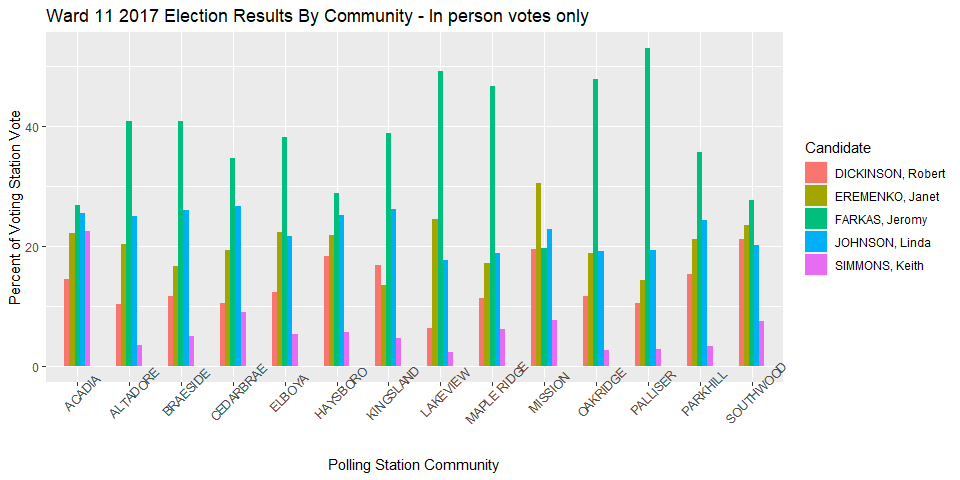
\includegraphics{CalgaryVotingTrends_files/figure-latex/Ward11-1.pdf}

Next steps: Take a look at those communities and overlay demographics
maybe add Mayor bars. compare to previous election, compare to
provincial and federal elections, compare to special voters and advance
voters, demographics from federal census?

\end{document}
